\section{An algorithm to decide type bisimilarity}
\label{sec:algorithm}

% Recall the type bisimulation problem for context-free session types.

% \begin{quote}
%   Given context-free session types $S$ and $T$, the type equivalence
%   problem consists in deciding if types $S$ and $T$ are equivalent,
%   i.e., $S \TypeEquiv T$.
% \end{quote}

This section presents an algorithm to decide whether two types are in
a type bisimulation. In the process we also provide an algorithm to
decide the equivalence of simple context-free languages.
%
The algorithm comprises three stages:
%
\begin{enumerate}
\item Translate the two types into a context-free grammar,
\item Prune unreachable symbols in productions, and
\item Explore an expansion tree, alternating between simplification
  and expansion operations, until either finding an empty node---case
  in which it decides positively---or failing to expand a node---case
  in which it decides negatively.
\end{enumerate}

\paragraph{Translating types to grammars}

% GREIBACH NORMAL FORMS

Type variables~$X$ are the \emph{non-terminal symbols} and LTS
labels~$a$ are the \emph{terminal symbols}. Sequences of type
variables~$\vec X$ are called \emph{words}; $\varepsilon$ denotes the
empty word.
%
A context-free grammar in Greibach normal form is a pair
$(\vec X,\mathcal P)$ where~$\vec X$ is the \emph{start word}
and~$\mathcal P$ a \emph{set of productions} of the form
$Y \rightarrow a\vec Z$ (context-free session types do not require
productions of the form $Y \rightarrow\varepsilon$).
%
Due to the deterministic nature of context-free session types, the
grammars we are interested in are \emph{simple}: for each
non-terminal symbol~$X$ and each terminal symbol~$a$, there is at most
one production of the form $X \rightarrow a\vec Y$.

% GRAMMAR LTS

Grammars in Greibach normal form naturally induce a labelled
transition system by taking words~$\vec X$ as states, terminal
symbols~$a$ as actions, and the transition relation $\LTSderivesP$,
defined as $X\vec Y\LTSderivesP \vec Z\vec Y$ when
$X \rightarrow a\vec Z \in \mathcal P$.  The associated bisimilarity
is denoted by $\ProdEquiv$.

% UNRAVEL

The \emph{unravelling} function on well-formed context-free session
types is defined as follows.
%
\begin{align*}
  \Unravel(\mu X.T) & = \Unravel\subs{\mu X.T}XT])
  \\
  \Unravel (S;T) &= \left\{%
  \begin{array}{ll}
    \Unravel(T) & \Unravel(S) = \skipk
    \\
    (\Unravel(S); T) & \Unravel(S) \ne \skipk
  \end{array}
                        \right.
  \\
  \Unravel (T) &= T \qquad \text{in all other cases}
  % \Unravel(\mu X.T) & = \Unravel\subs{\mu X.T}XT])
  % &
  % \Unravel (S;T) &= \Unravel(T) \quad (\Unravel(S) = \skipk)
  % \\
  % \Unravel (T) &= T \quad (\text{all other cases})
  % &
  % \Unravel (S;T) &=  \Unravel(S); T \quad (\text{otherwise})
\end{align*}
%
The function terminates under the assumption that types are well
formed. Thiemann and Vasconcelos~\cite{thiemann2016context} show that
$\Unravel$ yields a guarded type: $\skipk$, $\sharp B$,
$\star\{\ell_i\colon S_i\}$, or a $;$-type that starts with one the
these.

% TO GRAMMAR

Function $\word$ builds a word from a type. In the process it updates a
set $\productions$ of grammar productions. Word concatenation is
denoted by $\vec X\cdot\vec Y$.
%
\begin{align*}
  \word(\skipk) &= \Empty
  \\
  \word(S;T) &= \word(S) \cdot \word(T)
  \\
  \word(\sharp B) &=
    \productions := \productions \cup (Y \rightarrow \sharp B); Y
    \quad (Y\text{ fresh})
  \\
  \word(\star\{\ell_i\colon T_i\}_{i\in I}) &=
    \productions := \productions \cup \{Y \rightarrow\star l_i\cdot \word(T_i) \mid i\in I\}; Y
    \quad (Y\text{ fresh})
  \\
  \word(X) &= X
  \\
  \word(\mu X.T) &= X
\end{align*}

% COLLECT

Assume that $\{\mu X_1.T_1,\dots,\mu X_n.T_n\}$ is the set of all
$\mu$-subterms in a given type~$T$. Further assume that $i<j$ whenever
$X_i \in \free(\mu X_j.S_j)$. That is, the $\mu$-subterms are
topologically sorted with respect to their lexical nesting.
%
Now we identify unrolled versions of the $\mu$-subterms. Clearly, each
type $T_i$ is closed (has no free variables).
%
\begin{align*}
  T_1' &= \subs{\mu X_1.T_1}{X_1}{T_1} \\
  T_2' &= \subs{\mu X_2.T_2}{X_2}{ \subs{\mu X_1.T_1}{X_1}{T_2} }\\
       &\;\;\vdots \\
  T_n' &= \subs{\mu X_n.T_n}{X_n}{ \cdots \subs{\mu X_1.T_1}{X_1}{T_n} }
\end{align*}

% THE TRANSLATION

Finally, given an initial set of productions $\productions$, function
$\grm$ translates a type $T$ into a grammar composed of a start word
and set of productions:
%
\begin{equation*}
  \grm(T,\productions) = (\word(T),\; \productions \cup \{\word(\Unravel(T_1')), \dots \word(\Unravel(T_n'))\})
\end{equation*}

% The algorithm keeps the set of productions and an integer (to generate
% fresh non-terminal symbols) in the monadic state
% \lstinline{TransState}. It uses the following functions to manipulate
% state.
% %
% \begin{itemize}
% \item \lstinline{freshVar} returns a fresh non-terminal symbol (a type
%   variable);
% \item \lstinline{addProduction}$\,X\,a\,\vec Y$ updates the state by inserting
%   the production $X\rightarrow a\vec Y$;
% % \item \lstinline{insertVisited} marks a non-terminal symbol as visited;
% % \item \lstinline{isVisited} identifies whether the given non-terminal symbol
% %   was previously visited;
% % \item \lstinline{subst} $X\,T\,S$ replaces the occurrences of~$X$
% %   by~$T$ in~$S$;
% \item \lstinline|getTransitions|$\,X$ retrieves the transitions
%   from~$X$ (a map from terminal symbols~$a$ to words~$\vec Y$):
% \item \lstinline|reverseLookup| lookup a key for a value in the map.
% \end{itemize}

%\begin{lstlisting}[
  caption={Haskell code for stage 1: the conversion of types into grammars},
  label={lst:toGrammar},
  captionpos=b]
type Transitions = Map.Map LTSLabel [TypeVar]
type Productions = Map.Map TypeVar Transitions
type Visited = Set.Set TypeVar
type TransState = State (Productions, Int)

toGrammar :: Type -> TransState [TypeVar]
toGrammar Skip =
  return []
toGrammar (Message p b) = do
  y <- freshVar
  addProduction y (MessageLabel p b) []
  return [y]
toGrammar (Choice c m) = do
  y <- freshVar
  mapM_ (assocsToGrm y c) (Map.assocs m)
  return [y]
toGrammar (Semi t u) = do
  xs <- toGrammar t
  ys <- toGrammar u
  return (xs ++ ys)
toGrammar (Rec x t) = do
  zs <- toGrammar t
  if null zs
    then return []
    else do
      m <- getTransitions (head zs)
      addProductions x (Map.map (++ tail zs) m)
      return [x]
toGrammar (Var x) =
  return [x]

assocsToGrm :: TypeVar -> ChoiceView -> (TypeLabel,Type) -> TransState ()
assocsToGrm y c (l, t) = do
  xs <- toGrammar t
  addProduction y (ChoiceLabel c l) xs
\end{lstlisting}

%%% Local Variables:
%%% mode: latex
%%% TeX-master: "main"
%%% End:


Notice that $\grm$ terminates on all inputs (because recursion is
always on subterms) and adds a finite number of productions to the
original set. Furthermore, due to the deterministic nature of session
types, the function returns a simple grammar.
%
To run $\grm$ on two well-formed types proceed as follows: rename the
second type so that bound variables do not overlap with those of the
first; start with an empty set of productions; run the algorithm
consecutively on the two types to obtain two initial words and a
single set of productions.

\begin{example}
  \label{ex:productions}
  Consider the following pair of context-free session types.
  % 
  \begin{align*}
    S & \triangleq (\mu X_1. \&\{n: X_1;X_1;?\intk, \ell: ?\intk\});(\mu X_2. !\intk ; X_2;X_2)\\
    T & \triangleq (\mu Y_1. \&\{n: Y_1;Y_1, \ell: \skipk\};?\intk);(\mu Y_2. !\intk ; Y_2)
  \end{align*}
  % 
  Starting from the empty set of production, running $\grm$
  consecutively on~$S$ and on~$T$ produces the following set of
  productions
  %
  \begin{align*}
    X_1 &\rightarrow \& n\, X_1 X_1 X_3 & X_3 &\rightarrow \,? \intk &
    Y_1 &\rightarrow \& n\, Y_1 Y_1 Y_3 & Y_2 &\rightarrow \,!\intk\, Y_2 
    \\
    X_1 &\rightarrow \& \ell\, X_4           & X_4 &\rightarrow \,? \intk &
    Y_1 &\rightarrow \& \ell \,Y_3           & Y_3 &\rightarrow \,? \intk
    \\
    X_2 &\rightarrow \,!\intk\, X_2 X_2
  \end{align*}
  %
  and two start words $X_1X_2$ and $Y_1Y_2$.
\end{example}

\paragraph{Pruning unnormed productions}

For $\vec a$ a word $a_1,\dots, a_n$ ($n\ge1$), write
$\vec Y \LTSderivesP[\vec a] \vec Z$ when
$\vec Y \LTSderivesP[a_1] \cdots \LTSderivesP[a_n] \vec Z$.
%
We say that $\vec Y$ is \emph{normed} when
$\vec Y \LTSderivesP[\vec a] \varepsilon$ for some~$\vec a$, and that
$\vec Y$ is \emph{unnormed} otherwise.
%
When $\vec Y$ is normed, the \emph{minimal path} of $\vec Y$ is the
shortest~$\vec a$ such that $\vec Y \LTSderivesP[\vec a]
\varepsilon$.
%
In this case, the \emph{norm} of $\vec Y$, denoted by $|\vec Y|$, is
the length of~$\vec a$.
%
% Using the same approach as~\cite{DBLP:journals/iandc/ChristensenHS95} on
% the definition of (un)normed processes, we say that a sequence of symbols
% $\vec Y$ is \emph{normed} if there are labels $a_1,\ldots, a_n$
% such that:
% \begin{equation}
% \label{eq:path}
% 	\vec Y \rightarrow a_1\enspace Y_1 \rightarrow \cdots \rightarrow a_n
% 	\rightarrow \varepsilon.
% \end{equation}
% $\vec Y$ is said to be \emph{unnormed} when it is not normed. If $\vec Y$
% is normed, we define its \emph{norm} as:
% \[ | \vec Y | = \underset{n}{\mathsf{min}} \{\vec Y \rightarrow a_1\enspace Y_1
% \rightarrow \cdots \rightarrow a_n \rightarrow \varepsilon \}.\]
% A \emph{minimal path} for a normed sequence of symbols $\vec Y$ is a sequence of
% labels $\vec a = a_1,\ldots,a_n$ as in~\eqref{eq:path} such that
% $n = | \vec Y |$. To ease notation, we will also represent~\eqref{eq:path} as
% $\vec Y \xrightarrow{\vec a} \varepsilon$.
%
As observed by Christensen H\"uttel, and
Stirling~\cite{DBLP:journals/iandc/ChristensenHS95}, any unnormed word
$\vec Y$ is bisimilar to its concatenation with any other word, that
is, if $\vec Y$ is unnormed, then $\vec Y \ProdEquiv \vec Y \vec X$.
We use this fact to prune unreachable symbols in unnormed words. And
we do this in all productions as well as in the start words.

%The code is in Listing~\ref{lst:prune}.

% \begin{lstlisting}[
%   caption={Haskell code for stage 2: pruning unnormed productions},
%   label={lst:prune},
%   captionpos=b
%   ]
% type Visited = Set.Set [TypeVar]

% prune :: Productions -> Productions
% prune p = Map.map (Map.map (pruneWord p)) p

% pruneWord :: Productions -> Word -> Word
% pruneWord p = foldr (\x ys -> if normed p x then x:ys else [x]) []

% normed :: Productions -> TypeVar -> Bool
% normed p x = isJust $ maybeNorm p [x]

% maybeNorm :: Productions -> [TypeVar] -> Maybe Int
% maybeNorm p = norm Set.empty
%   where
%   norm :: Visited -> [TypeVar] -> Maybe Int
%   norm _ [] = Just 0
%   norm v xs
%    | any (flip isSubsequenceOf xs) v = Nothing
%    | otherwise = fmap (+1) (Map.foldr (compose min) Nothing (norms v xs))
%   norms :: Visited -> [TypeVar] -> Map.Map Label (Maybe Int)
%   norms v xs = Map.map (norm (Set.insert xs v)) (transitions xs p)
% \end{lstlisting}

\begin{example}
  \label{ex:prune}
  Recall Example~\ref{ex:productions} and notice that $X_2$ and $Y_2$
  are both unnormed. Then, the last occurrence of $X_2$ in production
  $X_2 \rightarrow \,!\intk\, X_2 X_2$ is unreachable, hence we
  simplify the production to obtain $X_2 \rightarrow \,!\intk\, X_2$.
  % \begin{center}
  %   \begin{tabular}{l l l}
  %     \multicolumn{3}{c}{Pruned productions for type $S$}\\ \hline
  %     \multicolumn{3}{c}{Start word: $X_1X_4$}\\
  %     $X_1 \rightarrow \& \ell\, X_3$  &
  %     $X_1 \rightarrow \& n\, X_1 X_1 X_2$ &
  %     $X_2 \rightarrow \,? \intk$ 
  %     \\
  %     $X_3 \rightarrow \,? \intk$ &
  %     $X_4 \rightarrow \,!\intk\, X_4$
  %   \end{tabular}
  % \end{center}
\end{example}

\paragraph{Building an expansion tree}

% We recall that, given two context-free session types $S$ and $T$, our main goal
% is to decide whether these types are equivalent or not. For this purpose,
% the algorithm we propose starts by applying algorithm presented in
% Listing~\ref{lst:toGrammar} to convert $S$ and $T$ into a grammar containing
% the productions derived from them. Afterwards, the algorithm in
% Listing~\ref{lst:prune} is used to streamline the grammars, by pruning
% unnormed sequences of symbols. Throughout this section we focus on the
% third and last step of the algorithm.

We base the third stage of the algorithm on the notion of
\emph{expansion tree} as proposed by Jan{\v{c}}ar and
Moller~\cite{janvcar1999techniques}, adapting an idea by
Hirshfeld~\cite{hirshfeld1996bisimulation}. The \emph{nodes} in trees
are labelled by sets of pairs of words.
%
We say that a node $N'$ is an \emph{expansion} of $N$ if $N'$ is a
minimal set such that: for every pair $(\vec X, \vec Y) \in N$,
\begin{itemize}
\item if $\vec X \rightarrow a\vec X'$ then
  $\vec Y \rightarrow a\vec Y'$ with $(\vec X',\vec Y')\in N'$, and
\item if $\vec Y \rightarrow a\vec Y'$ then
  $\vec X \rightarrow a \vec X'$ with $(\vec X',\vec Y')\in N'$.
\end{itemize}

An \emph{expansion tree} is built from a root node: the singleton set
containing the pair of start words obtained by translating the two
types into a grammar. Children nodes are obtained from their parent
node by expansion. Jan{\v{c}}ar and Moller observed that expansion
alone often leads to infinite trees. We then alternate between
expansion and simplification operations, until either finding an empty
node---case in which we decide equivalence positively---or failing to
expand a node---case in which we decide equivalence negatively.
%
% The na\"ive proposal for an expansion tree considers that any
% children node is obtained by expansion from its parent
% node. Nevertheless, as Jan{\v{c}}ar and Moller observed, this would
% often lead to infinite expansion trees. Hence, we follow the
% proposal in~\cite{janvcar1999techniques} and let the expansion tree
% alternate between simplification and expansion operations until
% either finding an empty node---case in which we decide equivalence
% positively---or failing to expand a node---case in which we decide
% equivalence negatively.
%
We say that a branch is \emph{successful} if it is infinite or
finishes in an empty node, otherwise it is said to be
\emph{unsuccessful}.

%\paragraph*{Expansion step}
In the \emph{expansion step}, each node $N$ derives a single child
node, obtained as an expansion of $N$. As we are dealing with simple
grammars, no branching is expected in the expansion tree at this
step.
%
% \paragraph*{Simplification step}
The \emph{simplification step} consists on the application of the
following rules:
%
\begin{description}
\item[Reflexive rule:] Omit from a node any pair of the form
  $(\vec X,\vec X)$;
\item[Congruence rule:] Omit from a node $N$ any pair that belongs to
  the least congruence containing the ancestors of $N$;
  % \item {\bf Basic Process Algebra rules:} create sibling nodes for $N$
  % according to the following rules:
  % \begin{description}
\item[BPA1 rule:] If $(X_0 \vec X, Y_0 \vec Y)$ is in
  $N$ and $(X_0 \vec {X'}, Y_0 \vec {Y'})$ belongs to the ancestors of
  $N$, then create a sibling node for $N$ replacing
  $(X_0 \vec X, Y_0 \vec Y)$ by $(\vec X, \vec {X'})$ and
  $(\vec Y, \vec {Y'})$;
\item[BPA2 rule:] If $(X_0 \vec X, Y_0 \vec Y)$ is in $N$
  and $X_0$ and $Y_0$ are normed, then:
  \begin{description}
  \item[Case $|X_0| \leq |Y_0|$:] Let $\vec a$ be a minimal path
    for $X_0$ and $\vec Z$ the word such that
    $ Y_0 \LTSderivesP[\vec a] \vec Z$. Add a sibling node for
    $N$ including the pairs $(X_0 \vec Z, Y_0)$ and
    $(\vec X, \vec Z \vec Y)$ in place of $(X_0 \vec X, Y_0 \vec Y)$;
%  \item[Case] $|X_0| > |Y_0|$: Let $\vec a$ be a minimal path for 
  \item[Otherwise:] Let $\vec a$ be a minimal path for 
    $Y_0$ and $\vec Z$ the word such that
    $ X_0 \LTSderivesP[\vec a] \vec Z$. Add a sibling node for $N$
    including the pairs $(X_0 , Y_0 \vec Z )$ and
    $(\vec Z\vec X, \vec Y)$ in place of $(X_0 \vec X, Y_0 \vec Y)$.
  \end{description}
%		  \end{description}
%	\item {\bf Filtering rule:} remove any node containing a pair
%	       $(\vec X, \vec Y)$ such that $|\vec X|\neq |\vec Y|$.
\end{description}

Contrarily to expansion and to the reflexive and congruence
simplifications, \BPA\ rules promote branching in the expansion
tree. The number of children nodes generated by these rules is
finite~\cite{DBLP:journals/iandc/ChristensenHS95}.
%
Notice that the sibling nodes do not exclude the (often) infinite
branch resulting from successive expansions.

\paragraph{Checking the bisimilarity of context-free session types}

Given a set of productions and two start words $\vec X$ and $\vec Y$
(all pruned), function $\Bisim$ alternates between simplification and
expansion stages, starting with simplification.
%
To avoid getting stuck in an infinite branch of the expansion tree, we
use a breadth-first search on the expansion tree: node-ancestors pairs
to be processed are stored in a queue. The initial pair contains the
initial node $\{(\vec X,\vec Y)\}$ and the empty set of ancestors.
%
\begin{equation*}
  \Bisim(\vec X, \vec Y) = \simplify((\{(\vec X,\vec Y)\},\emptyset), \mathsf{emptyQueue})
\end{equation*}

The simplification stage distinguishes the case where all type
variables are normed, in which case \BPA1 is not required to decide
equivalence~\cite{caucal1986decidabilite,DBLP:journals/iandc/ChristensenHS95},
from the case where some type variables might be unnormed.
%
\begin{align*}
  \mathsf{rules} =\;& \If\ \mathsf{allProductionsNormed}\ \Then\
  [\mathsf{reflex} ,\mathsf{congruence}, \mathsf{bpa2}]\\
  &\Else\ [\mathsf{reflex} ,\mathsf{congruence}, \mathsf{bpa1} , \mathsf{bpa2}]
\end{align*}

Predicate $\simplify$ applies the various $\mathsf{rules}$ and then
calls function $\expand$.
%
The application of each rule (function $\mathsf{apply}$) produces a
set of node-ancestors pairs that are enqueued.
%
\begin{align*}
  &\simplify(\mathit{na}, q) = \expand(\Fold(\mathsf{append}, q,
    \Fold(\mathsf{apply}, \mathit{na}, \mathsf{rules})))
\end{align*}

Predicate $\expand$ terminates as soon as all nodes fail to expand
and, thus, the queue is empty, case in which the algorithm returns
$\False$, or an empty node is reached, case is which the algorithm
returns $\True$.
%
\begin{align*}
  &\expand(q) =\\
  &\quad \If\ \mathsf{empty}(q)\ \Then\ \False\\
  &\quad \Else\ (n,a) = \mathsf{front}(q)\\
  & \qquad\quad\; \If\ \mathsf{empty}(n)\ \Then\ \True\\
  & \qquad\quad\; \Else\ \If\ \mathsf{hasChild}(n)\ \Then\
    \simplify(\mathsf{child}(n), a \cup n, \mathsf{dequeue}(q))\\
  & \qquad\qquad\quad\;\: \Else\ \expand(\mathsf{dequeue}(q))
\end{align*}

% Given two context-free session types, function \lstinline|bisimilar|
% (in Listing~\ref{lst:algorithm}) starts by converting the two session
% types into a grammar, which is then pruned. Function
% \lstinline|convertToGrammar| (in Appendix) builds the initial monadic
% state, and runs the algorithm in Listing~\ref{lst:toGrammar} to
% convert the session types given as parameters.
% %
% An expansion tree is computed afterwards, through an alternation of
% expansion of children nodes and their simplification, using the
% reflexive, congruence, and \BPA\ rules.
% %
% \begin{lstlisting}[
%   caption={Haskell code for checking the bisimilarity of context-free
%     session types},
%   label={lst:algorithm},
%   captionpos=b
%   ]
% type Node = Set.Set (Word, Word)
% type Ancestors = Node
% type NodeQueue = Queue.Seq (Node, Ancestors)

% bisimilar :: TypeEnv -> Type -> Type -> Bool
% bisimilar tEnv t u = expand (xs, ys) (prune p)
%   where Grammar [xs, ys] p = trace (show t ++ "\nbisim\n" ++ show u) $ convertToGrammar tEnv [t, u]
        
% expand :: (Word, Word) -> Productions -> Bool
% expand p = expand' 1 (Queue.singleton (Set.singleton p, Set.empty))
%   where
%   expand' :: Int -> NodeQueue -> Productions -> Bool
%   expand' i ((n, a) Queue.:<| q) ps
%     | Set.null n      = True
%     | otherwise       = case expandNode ps n of
%         Nothing -> expand' (i+1) q ps
%         Just n' -> expand' (i+1) (simplify i ps n' (Set.union a n) q) ps
%   expand' _ Queue.Empty _ = False

% simplify :: Int -> Productions -> Node -> Ancestors -> NodeQueue -> NodeQueue
% simplify i ps n a q =
%   foldr enqueueNode q nas'
%   where nas' = if allNormed ps
%                then foldr (apply ps) nas [reflex,congruence,bpa2]
%                else foldr (apply ps) nas [reflex,congruence,bpa1,bpa2]

% enqueueNode :: (Node,Ancestors) -> NodeQueue -> NodeQueue
% enqueueNode (n,a) q = q Queue.|> (n,a)
% \end{lstlisting}
% type NodeTransformation = Productions -> Ancestors -> Node -> Set.Set Node 

\begin{example}
  The expansion tree for our running example is in the diagram
  below. Once a successful branch is reached (the $\checkmark$ in the
  figure), $\Bisim(\vec X, \vec Y)$ returns $\True$. \vv{adjust the
    variables in the diagram according to new grammar in example 1}
  \begin{center}
    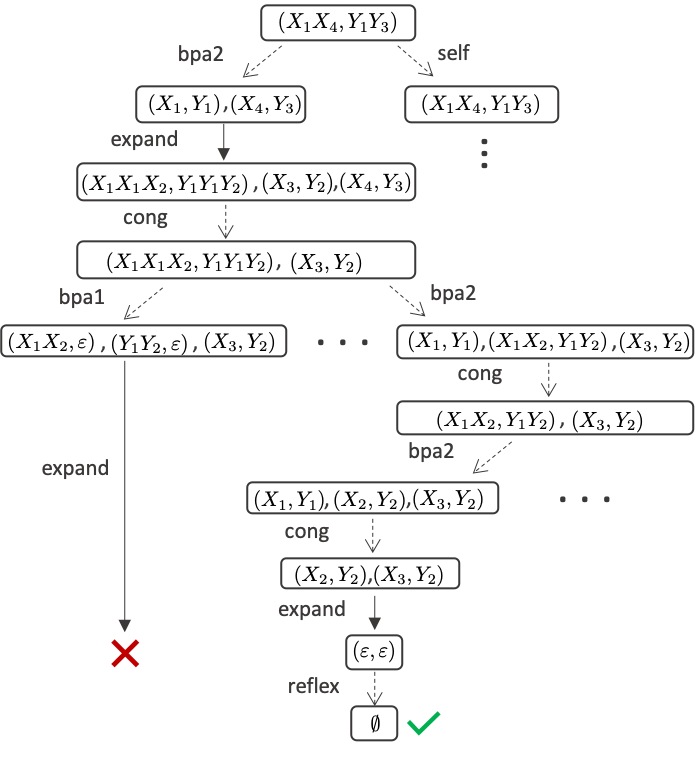
\includegraphics[width=7.5cm]{img/expansionTree}
  \end{center}
\end{example}

%%% Local Variables:
%%% mode: latex
%%% TeX-master: "main"
%%% End:
